% Определение класса для файла
\documentclass[12pt, times]{article} % размер 12, шрифт Times New Roman

% Подключение файла с настройками и подключенными пакетами
% Макет страницы
\usepackage[a4paper, left=3.5cm, right=1.5cm, top=2cm, bottom=2cm]{geometry} % подключает пакет geometry для управления размерами страницы
\usepackage[onehalfspacing]{setspace} % 1.5 интервал
\usepackage{indentfirst} % добавляет отступ для абзаца после секции

% Настрока заголовков и подзаголовков для оглавления
\usepackage{titlesec}

% Настройка \section: шрифт 14pt, выравнивание по центру
\titleformat{\section}
  {\normalfont\fontsize{14}{16}\selectfont\bfseries\centering} % стиль шрифта заголовка
  {} % без номера в тексте, но номер будет в ToC
  {0pt} % расстояние между номером и заголовком
  {} % код перед названием секции
% Отступ слева = абзацный отступ, сверху = 2 строки, снизу = 1 строка
\titlespacing*{\section}
  {0pt} % левый отступ не нужен
  {2ex} % отступ сверху
  {1ex} % отступ снизу

% Настройка \subsection: шрифт 12pt, выравнивание по абзацу
\titleformat{\subsection}
  {\normalfont\fontsize{12}{14}\selectfont\bfseries} % стиль шрифта подзаголовка
  {} % без номера в тексте, но будет номер в ToC
  {0pt} % расстояние между номером и заголовком
  {} % код перед названием

\titlespacing*{\subsection}
  {\parindent} % левый отступ как у абзаца
  {3ex} % отступ сверху
  {1ex} % отступ снизу

% Настройка \subsubsection: шрифт 12pt, выравнивание по абзацу
\titleformat{\subsubsection}
  {\normalfont\fontsize{12}{14}\selectfont\bfseries} % стиль шрифта подзаголовка
  {} % без номера в тексте, но будет номер в ToC
  {0pt} % расстояние между номером и заголовком
  {} % код перед названием

\titlespacing*{\subsubsection}
  {\parindent} % левый отступ как у абзаца
  {3ex} % отступ сверху
  {1ex} % отступ снизу

% Настройки внутри списков
\usepackage{enumitem}

% Добавляем точки в оглавление
\usepackage{tocloft}
\renewcommand{\cftsecleader}{\cftdotfill{\cftdotsep}} % добавляем точки
\renewcommand{\cftdotsep}{1} % плотность точек

% Кодировка и поддержка кириллицы
\usepackage[utf8]{inputenc} % позволяет использовать текст в кодировке UTF-8
\usepackage[T2A]{fontenc} % поддержка русских шрифтов (кириллица)
\usepackage[english, russian]{babel} % включение правил типографики для английского языка (переносы, заголовки и т.д.)

% Кавычки и цитаты
\usepackage{csquotes} % поддержка корректного форматирования кавычек и цитат (особенно важно при использовании biblatex)

% Вставка изображений
\usepackage{graphicx} % позволяет вставлять и масштабировать изображения (\includegraphics)

%\begin{figure}[htbp] % here, top, bottom, page
%    \centering
%    \includegraphics[width=0.8\textwidth]{имя_файла.png}
%    \caption{Подпись к рисунку}
%    \label{fig:example}
%\end{figure}

% Указание папки для поиска изображений
\graphicspath{{images/}}

% Таблицы
\usepackage{array} % расширенные возможности для работы с таблицами
\usepackage{tabularx} % автоматический подбор ширины столбцов

\usepackage{multirow} % настройка для множественных строк
\renewcommand{\arraystretch}{1.0} % размер между строк таблиц, 1.0 по умолчанию

\usepackage{longtable} % позволяет создавать таблицы, которые переносятся на следующие страницы
\usepackage{etoolbox} % нужен для двух следующих команд
\AtBeginEnvironment{table}{\fontsize{10}{10}\selectfont} % для изменения размера шрифта меняем первое значение в {}
\AtBeginEnvironment{longtable}{\fontsize{10}{10}\selectfont} % для изменения размера шрифта меняем первое значение в {}

% Математические выражения
\usepackage{amsmath, amssymb} % расширенные математические окружения; дополнительные математические символы

% Ссылки
\usepackage[
    colorlinks=true, % включение цвета для ссылок
    linkcolor=black, % цвет оглавления
    urlcolor=blue, % цвет url-ссылок в тексте и библиографии
    citecolor=black % цвет для текста в цитатах
]{hyperref} % добавляет активные гиперссылки на разделы, рисунки, библиографию и внешние URL

% Подписи к картинкам и таблицам
\usepackage[justification=centering]{caption} % более гибкое управление подписями к рисункам и таблицам
\captionsetup[table]{labelfont=bf, textfont=bf} % textfont=normalfoint для обычного шрифта в тексте таблиц
\captionsetup[figure]{labelfont=bf, textfont=bf} % textfont=normalfoint для обычного шрифта в тексте картинок
\usepackage{subcaption} % позволяет делать несколько подрисунков с подписями (a), (b), ...

% Библиография
\usepackage[backend=biber, style=gost-numeric, autolang=other, sorting=none]{biblatex}
% использование biber для обработки ссылок
% ГОСТ-стиль нумерованной библиографии
% язык библиографии подбирается автоматически, нужно поле langid = {russian} или langid = {english} в .bib файле
\addbibresource{bib/bibliography.bib}
% заменим ; на запятую между несколькими ссылками
\renewcommand*{\multicitedelim}{\addcomma\space}

\begin{document}

% Титульный лист
\newpage
\begin{titlepage}

\begin{center}
    САНКТ-ПЕТЕРБУРГСКИЙ ГОСУДАРСТВЕННЫЙ УНИВЕРСИТЕТ \\КАФЕДРА ГЕНЕТИКИ И БИОТЕХНОЛОГИИ
    \vspace{5cm}

    % Автор
    \textbf{Васильев Артем Викторович \\Выпускная квалификационная работа}
    \vspace{1cm}

    % Название работы
    ``Эволюционные особенности структуры гена \\\textit{Nxf1} (nuclear export factor) у животных``
\end{center}

\vfill

\begin{flushright}
    Научный руководитель: \\к.б.н., доцент, кафедра генетики и биотехнологии, \\Голубкова Елена Валерьевна \\
    \vspace{1cm}
    Рецензент: \\заведующая лабораторией, ведущий научный сотрудник, \\лаборатория эволюционной геномики и палеогеномики, ЗИН, \\к.б.н., с.н.с., \\Абрамсон Наталья Иосифовна
\end{flushright}

\vfill

\begin{center}
    Санкт-Петербург \\2025
\end{center}

\end{titlepage}

\setcounter{page}{2} % изменение номера СЛЕДУЮЩЕЙ страницы


% Аннотация
% \input{chapters/annotation}

% Оглавление
\newpage
\renewcommand{\contentsname}{\centerline{\large Оглавление}}
\tableofcontents


% Список использованных сокращений
% \input{chapters/abbreviations}

% Введение
% \clearpage
\section{Введение}

Для большинства генов высших эукариот характерна мозаичная структура, в составе которой выделяют кодирующие участки экзоны и некодирующие - интроны.
В процессе созревания транскрипта интроны, как правило, вырезаются сплайсингом, и из ядра выходят мРНК, лишенные интронных последовательностей.
Однако альтернативный сплайсинг позволяет получать несколько различных зрелых мРНК из одной пре-мРНК, что значительно расширяет протеом без увеличения числа генов.

Особый интерес представляют транскрипты, сохраняющие интрон (intron retention, IR): в таких первичных транскриптах интрон, обычно несущий преждевременный стоп-кодон, остается невырезанным, образуя устойчивую вторичную структуру, которая препятствует распознаванию факторами нонсенс-опосредованного распада (nonsense mediated mRNA decay, NMD) и впоследствии обеспечивает синтез укороченного, но функционально значимого белка~\cite{Mamon2019}.

Однако, несмотря на наличие специфического механизма, среди различных групп, эволюционно далеких друг от друга, описаны случаи существования транскриптов с сохраненным интроном.
Отдельно можно выделить модельный объект \textit{Drosophila melanogaster} и человека, для которых известно семейство генов \textit{Nxf} (nuclear export factor), в котором нас заинтересовал ген \textit{Nxf1}.
Данный ген кодирует белок, являющийся основным транспортером мРНК из ядра в цитоплазму.

У гена \textit{Nxf1} (nuclear export factor 1), кодирующего основной транспортер мРНК из ядра в цитоплазму, существует так называемая ``консервативная кассета``, которая включает два коротких экзона (110 и 37 нуклеотидов в каноническом варианте) и ``кассетный`` интрон между ними.
Названия сформулированы нашей научной группой.
Эта структура сохраняется также и у представителей других филогенетических групп: благодаря образованию специфической вторичной структуры или наличию в последовательности интрона специфических последовательностей, например конститутивного транспортного элемента (constitutive transport element, CTE), транскрипт, содержащий преждевременный стоп-кодон, избегает NMD и кодирует укороченную форму белка.

Анализ подобных транскриптов показал, что консервативные элементы ``кассеты`` \textit{Nxf1} специфичны для разных клад организмов, а интрон-содержащие транскрипты формируют уникальные вторичные структуры, что подчеркивает эволюционную и функциональную значимость интронов.

Научная новизна работы заключается в сравнительном анализе структуры гена \textit{Nxf1} у представителей различных филогенетических групп, данных по которым ранее не было, с целью выявления закономерностей эволюции нуклеотидной и белковой последовательности гена \textit{Nxf1}.
В бакалаврской работе было показано, что ``консервативная кассета`` сохраняет свойства внутри артропод, особенно внутри семейства Drosophilidae, однако вопрос о степени консервативности и специфике структурных элементов у более широкого круга организмов остается открытым.
Помимо сравнительного анализа последовательностей, важной частью исследования является построение вторичных структур интрон-содержащих транскриптов и выявление консервативных мотивов внутри интрона, способствующих его сохранению и избеганию нонсенс-опосредованного распада.


\subsection{Цель работы}

Изучить структуру гена \textit{Nxf1} у представителей разных филогенетических групп животных для выявления эволюционных закономерностей и особенностей ``кассетной`` структуры, а также проанализировать вторичные структуры интрон-содержащих транскриптов.


\subsection{Задачи}

\begin{enumerate}[left=\parindent]
  \item Найти нуклеотидные и аминокислотные последовательности гена \textit{Nxf1} у различных групп животных.
  \item Произвести поиск ``консервативной каасеты`` в нуклеотидной последовательности гена у найденных организмов.
  \item Выполнить анализ структуры, сравнить полученные последовательности между собой.
  \item Выявить и охарактеризовать консервативные участки ``кассетного`` интрона и прилегающих экзонов у видов из исследуемых таксонов.
  \item Провести анализ вторичной структуры интрон-содержащих транскриптов и оценить консервативные мотивы внутри интрона, потенциально способствующие его сохранению.
\end{enumerate}


% Обзор литературы
%%\clearpage
%\section{Обзор литературы}
%
%\subsection{Механизмы усложнения организации генома}
%
%Помимо стандартного варианта созревания РНК путем сохранения экзонов и сплайсосомного вырезания интронов из первичного транскрипта, существуют варианты, отличающиеся от канонического.
%Одним из таких вариантов является альтернативный сплайсинг - основной источник транскрипционной изменчивости, когда одному гену может соответствовать несколько транскриптов.
%Кроме общеизвестного ``удержания интрона`` (intron retention (IR)), важно обозначить такой процесс, как альтернативное полиаденилирование, так как оно также оказывает прямое влияние на вариативность транскриптов~\cite{Mamon2019}.
%
%Альтернативный сплайсинг (alternative splicing (AS)) достаточно распространен у эукариот.
%Данный механизм способствует увеличению белкового разнообразия у организма.
%Выделяют следующие типы альтернативного сплайсинга: т.н. ``пропуск экзонов``; вариант, когда используются наборы из нескольких экзонов, расположенных рядом друг с другом и  формирующих кассеты, при этом во время сплайсинга выбирается только один из нескольких экзонов в каждой из кассет; также могут использоваться различные 5'- и 3'-сайты сплайсинга в интронах или экзонах, выбор которых зависит от цис- и транс-действующих факторов, необходимых для формирования сплайсосомы~\cite{Mamon2019}.
%
%``Удержание интрона`` является одним из вариантов альтернативного сплайсинга, который распространен у млекопитающих.
%Данный механизм увеличивает сложность транскриптома~\cite{Schmitz2017}, но часто в интронах присутствуют кодоны преждевременной терминации (premature termination codons (PTCs)) внутри основной открытой рамки считывания.
%В результате возможно 2 исхода: нонсенс-опосредованный распад мРНК с сохраненным интроном или продукция укороченных белков~\cite{Mamon2019}.
%Именно эти варианты интересуют нас больше всего.
%Такие мРНК с оставшимся интроном дают альтернативные формы белков, а значит являются источником функционального разнообразия генных продуктов, что демонстрирует важность интронов как структурной единицы гена.
%Для разных организмов показано, что наличие такой мРНК с интроном для гена \textit{Nxf1} является консервативным признаком~\cite{Mamon2013}, о чем речь пойдет далее.
%
%
%\subsection{Значимость интронов}
%
%Интроны делят на 3 группы: I, II, III.
%Интроны I и II группы обнаруживаются в геномах некоторых бактерий и органелл.
%Интроны I группы также обнаружены в рибосомных РНК (рРНК) ядер протистов и грибов.
%Эти две группы имеют разные структуры РНК, которые облегчают их активность самосплайсинга.
%Они также содержат внутренние открытые рамки считывания (open reading frame (ORF)), которые облегчают как удаление интронов из транскриптов РНК, так и распространение интронов на безинтронные сайты посредством обратной транскрипции~\cite{Roy2006}.
%Третья же группа интронов – сплайсосомные интроны – найдены в ядерных геномах всех охарактеризованных эукариот.
%Обычно они не имеют открытых рамок считывания и их удаление происходит с помощью сплайсосомы~\cite{Jurica2013}.
%
%К непосредственным функциям интронов можно отнести следующее.
%Во-первых, это положительная регуляция экспрессии генов.
%Впервые данное явление было продемонстрировано очень давно в эксперименте с использованием конструкций вируса SV40, где показали, что количество белка было значительно снижено без его интронов~\cite{Gruss1979}.
%В последующем это было также показано на дрожжах и млекопитающих~\cite{Juneau2006}.
%
%Во-вторых, можно отнести регуляцию нонсенс-опосредованного распада мРНК, который был упомянут при описании удержания интрона.
%Обычно NMD описывают, как механизм надзора у эукариот, который избирательно удаляет мРНК, содержащие ошибочно сгенерированные PTCs~\cite{Jo2015}.
%Однако, есть доказательства в пользу того, что интроны, расположенные в 5'- или 3'-нетранслируемых областях (untranslated region (UTR)), играют важную роль в контроле NMD-чувствительности транскриптов~\cite{Kalyna2012}.
%
%В-третьих, интроны могут быть связаны с транспортом мРНК.
%Раньше считалось, что сплайсированные транскрипты быстрее экспортируются из ядра в цитоплазму, однако были и противоречивые исследования~\cite{Jo2015}.
%Один из относительно недавних экспериментов с использованием флуоресцентной гибридизацией in situ (FISH) показал, что несущие интроны транскрипты преимущественно расположены в цитоплазме~\cite{Valencia2008}, что сильнее подвергает сомнению высказанные ранее гипотезы и требует их пересмотра.
%
%Помимо перечисленных функций есть также предположение о том, что часть последовательностей концов интронов может быть ответственна за истощение нуклеосом в интронах путем отталкивания нуклеосом в сторону экзонов~\cite{Schwartz2009}.
%Это позволяет задуматься о роли интронов в сборке хроматина.
%
%Стоит отметить порядковое положение интронов в гене.
%Больше всего внимание привлекает первый интрон среди всех интронов гена, обычно именно он обладает особыми функциональными характеристиками~\cite{Jo2015}.
%Например, первый интрон гена \textit{oskar} Drosophila играет важную роль в правильной цитоплазматической локализации некоторых мРНК~\cite{Siemens2004}.
%
%Длина интронов также является важной характеристикой.
%Есть предположение о том, что длинные интроны повышают эффективность естественного отбора, устраняя интерференцию Хилла-Робертсона~\cite{Comeron2008}.
%
%В одной из работ десятилетней давности на дрожжах \textit{Saccharomyces cerevisiae} наблюдали, как короткие ORF могут эволюционировать в настоящие функциональные гены посредством своего рода непрерывного эволюционного процесса~\cite{Carvunis2012}.
%Это позволило предположить, что интроны могут стать источником новых генов.
%
%В наше время активно используется метод полногеномного поиска ассоциаций, сокращенно GWAS – genome-wide association study.
%В основе метода лежит сравнительный анализ однонуклеотидных вариантов (single-nucleotide variant (SNV)), а точнее участков в геноме, которые схожи между собой по этим однонуклеотидным заменам, между индивидуумами~\cite{Smith2019}.
%Примечательно, что при картировании аллелей, ассоциированных с какими-то заболеваниями, место картирования соответствует именно интронным областям~\cite{Welter2014}.
%Данный факт является очередным подтверждением важности изучения интронов.
%
%
%\subsection{Семейство генов \textit{Nxf}, общая характеристика}
%
%Принимая во внимание все выше сказанное, можно перейти к описанию основного объекта, на который направлено данное исследование.
%Перед этим стоит сказать несколько вводных слов про само семейство.
%
%Семейство генов \textit{Nxf} (nuclear export factor) было названо в честь функции универсального гена \textit{Nxf1}, продукт которого ответственен за ядерно-цитоплазматический транспорт большинства мРНК.
%Гены данного семейства обнаружены у всех эукариотических организмов группы Opisthokonta и характеризуются эволюционной консервативностью~\cite{Mamon2013}.
%
%Геномы различных грибов имеют лишь один ген-представитель этого семейства, растения и некоторые простейшие вовсе их лишены.
%Животные, как правило, имеют от двух до пяти паралогичных генов~\cite{Mamon2013}.
%
%Характерной особенностью для гена Nxf1 является существование транскриптов с невырезанным гомологичным интроном.
%Особое внимание выделяется консервативному блоку, состоящему из последовательно идущих экзонов размером 110 п.н. и 37 п.н., а также интрону, который находится между ними и который принято называть ``кассетным``~\cite{Mamon2013}.
%Соответственно, сам блок из трех единиц мы будем называть ``консервативной кассетой``.
%
%Среди животных, для которых есть данные про семейство генов Nxf, были выявлены 3 таксономические группы, и в каждой из них кассетный интрон имеет определенные характеристики~\cite{Mamon2013}.
%
%К первой группе относятся позвоночные, для них характерен интрон, находящийся между 10-м и 11-м экзонами в гене \textit{Nxf1}.
%В интроне позвоночных выявили 4 участка протяженной гомологии: 1) 5´-концевая последовательность; 2) фрагмент, содержащий конститутивный транспортный элемент (constitutive transport element (СТЕ), характерный для ретровирусов; 3) третий консервативный участок; 4) 3´-концевая последовательность~\cite{Mamon2013}.
%
%Ко второй группе принадлежат дрозофилиды с кассетным интроном 5-м в генах \textit{Nxf1}.
%Несмотря на отсутствие участков протяженной гомологии, что характерно для позвоночных, у разных видов Drosophilidae есть схожая черта – две протяженные последовательности, обогащенные аденином (А).
%Предполагается, что вторичная структура транскриптов с сохраненным интроном, образовавшаяся за счет наличия этих последовательностей, способствует их сохранению~\cite{Mamon2013}.
%
%В последнюю группу включены нематоды с интроном 5-м или 6-м.
%Его размер на порядок меньше, а участки протяженной гомологии не обнаружены.
%Однако, внутри группы есть общее сходство – это повышенное содержание тимина (Т), что отличает данную группу организмов от остальных~\cite{Mamon2013}.
%
%Как уже упоминалось ранее, важной особенностью для генов Nxf1 у позвоночных и дрозофилид является способность к образованию сложных вторичных структур, которая может играть существенную роль в пост-транскрипционной судьбе транскрипта~\cite{Golubkova2012}.
%Помимо этого, все же главной особенностью, кроме сохраненного интрона в транскрипте, становится наличие в этом сохранившемся интроне преждевременного стоп-кодона, но мРНК избегает нонсенс-опосредованного распада, и в итоге возможно образование укороченного белка.
%Перейдем к подробному рассмотрению гена \textit{Nxf1}.
%
%
%\subsection{Структура и функции Nxf1 (гена и белка)}
%
%Первоначально белок Nxf1 у людей был идентифицирован как потенциальный цитоплазматический кофактор для Tip (белок, взаимодействующий с тирозинкиназой), кодируемый вирусом герпеса saimiri, и был назван TAP (Tip-associated protein, или белок, ассоциированный с Tip)~\cite{Yoon1997}.
%Позже было показано, что ТАР участвует в ядерно- цитоплазматическом транспорте несплайсированной или частично сплайсированной РНК ретровирусов.
%TAP напрямую распознает только одну последовательность – CTE, которая была первоначально обнаружена в РНК ретровирусов~\cite{Zolotukhin2001}.
%Мы предполагаем, что функцию CTE у дрозофилид выполняет образуемая благодаря сохранению интрона вторичная структура.
%На данный момент наилучшее представление о гене \textit{Nxf1} есть для дрозофилид и млекопитающих.
%Рассмотрим функцию и организацию данного гена, а также белковые домены для \textit{Drosophila melanogaster} и \textit{Homo sapiens}.
%
%Nxf1 имеет модульную доменную организацию (на Рис.~\ref{fig:dm_hs_nxf1_structure} представлена структура гена, последовательности в котором кодируют белковую структуру), состоящую из РНК-связывающего домена (RBD), четырех богатых лейцином повторов (LRR), домена, проявляющего сходство с ядерным транспортным фактором 2 (NTF2-подобный домен), и С-концевой убиквитин-ассоциированный, или UBA-подобный, домен~\cite{Mamon2013}.
%
%\begin{figure}[h] % here, top, bottom, page
%    \centering
%    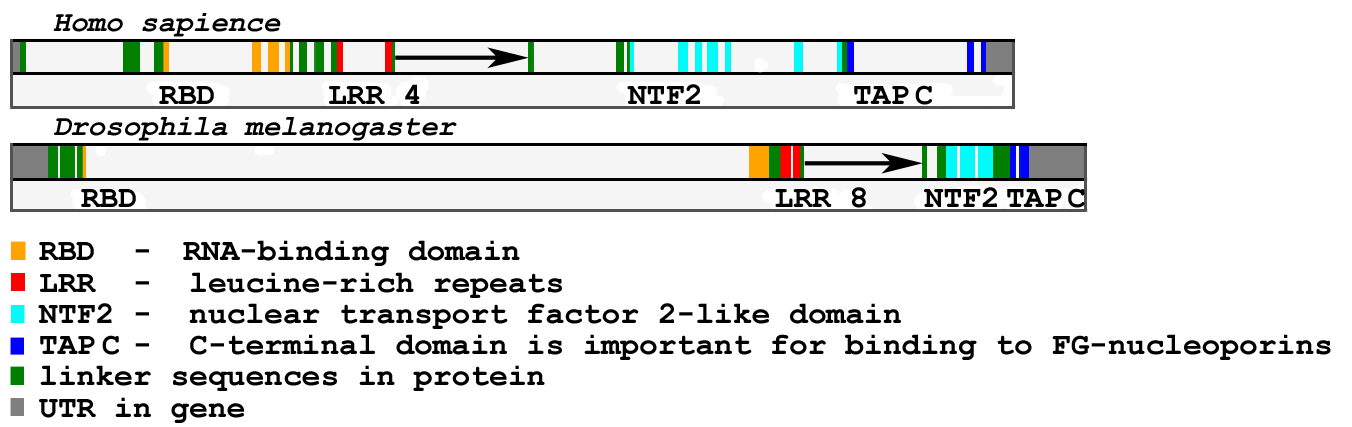
\includegraphics[width=0.9\textwidth]{images/dm_hs_nxf1_structure}
%    \caption{Интрон-экзонная структура для генов \textit{Hs Nxf1} и \textit{Dm Nxf1}. Стрелки обозначают ``кассетный`` интрон. Цвета экзонов отображают белковые домены~\cite{Mamon2013}.}
%    \label{fig:dm_hs_nxf1_structure}
%\end{figure}
%
%Основной и общеизвестной функцией продукта гена \textit{Nxf1} является транспорт всех типов мРНК из ядра в цитоплазму~\cite{Herold2000}.
%Кассетный интрон условно разделяет \textit{Nxf1} на две функциональные половины – рецепторную, куда относятся RBD и LRR, отвечающую за взаимодействие с РНК, и транспортную, куда входят NTF2L и UBA, позволяющую, взаимодействуя с другими белками, обеспечивать транспорт комплекса макромолекул через ядерные поры~\cite{Mamon2013}.
%
%Помимо классической функции нашей группой выявлены дополнительные, жизненно важные функции продукта гена \textit{Nxf1}, или \textit{sbr} у дрозофилид.
%Во-первых, доказано, что sbr выполняет семенниково-специфические функции.
%Показано, что существуют специфичные для семенников альтернативные транскрипты, полученные за счет альтернативного промотора, этого гена и укороченный белок sbr, обнаруженный только в семенниках~\cite{Ginanova2016}.
%
%Во-вторых, установлено, что белок sbr необходим для формирования внутренней структуры и установления границ в мозговом веществе зрительной системы дрозофилы.
%Распределение sbr в ядре и цитоплазме специфических нейронов и глиальных клеток свидетельствует о специализированных функциях этого белка~\cite{Mamon2021}.
%
%Также в одной из недавних работ была продемонстрирована значимость ``кассетного`` интрона в эволюции гена \textit{Nxf1} у представителей Chiroptera~\cite{Bondaruk2022}.
%
%В моей бакалаврской работе было проанализировано 89 нуклеотидных последовательностей гена \textit{Nxf1} из таксономической группы Arthropoda, а также найдены последовательности гена для 37 представителей дрозофилид.
%По результатам проведенных множественных выравниваний и построенных вторичных структур интрон-содержащего транскрипта были сформулированы следующие выводы:
%
%\begin{enumerate}[left=\parindent]
%    \item Структура ``консервативной кассеты`` является специфической для таксонов низкого ранга у всех взятых в анализ артропод.
%    \item Интрон-содержащие транскрипты формируют специфические вторичные структуры; у дрозофилид продемонстрировано наличие А-обогащенных участков.
%\end{enumerate}
%
%Таким образом, важность роли гена \textit{Nxf1} и ``кассетного`` интрона в нем не вызывает сомнений.
%Тем не менее очень интересно было бы проанализировать структуру данного гена у представителей за пределами Arthropoda, используя современные методы биоинформатики, освоенные в магистратуре, о чем и пойдет речь далее.


% Материалы и методы
\newpage
\section{Материалы и методы}

\subsection{Первичный анализ}

В качестве отправной точки был произведен поиск гена \textit{Nxf1} внутри веб-сервиса NCBI~\cite{ncbi_general}.
Полученные данные были сохранены в текстовом формате и загружены в виде tsv-таблицы с помощью пакета pandas v2.2.3~\cite{pandas} для языка программирования Python v3.12.6~\cite{python_3_12}.
Всего был найден 651 вид, содержащий анализируемый ген, большинство из которых относятся к Deuterostomia (Вторичноротые) – 436 видов.
Таким образом, в качестве материалов выступали нуклеотидные и белковые последовательности, соответствующие гену \textit{Nxf1}, из открытых баз данных NCBI~\cite{ncbi_general}.

Большинство этапов последующего анализа реализовано в виде отдельных скриптов, разработанных в рамках данной работы, если не указано другое.
Для логического разделения на блоки был использован Jupyter Notebook v1.1.1~\cite{jupyter_notebook}.

По данным из полученной таблицы в порядке поискового эксперимента было построено филогенетическое дерево по найденным видам для оценки количества видов в таксонах более низкого ранга.
Для глубокого анализа было принято решение сфокусироваться на организмах, относящихся к группе Protostomia (Первичноротые), Cnidaria (Стрекающие), а также на всех группах из Deuterostomia за исключением Mammalia (Млекопитающие).

\subsection{Загрузка данных}

Для найденных организмов с помощью пакета NCBI E-utilities из BioPython v1.85~\cite{biopython} и NCBI Datasets Command-Line Interface (CLI) v18.0.2~\cite{datasets} были загружены нуклеотидные последовательности гена, кодирующих участков и мРНК, а также аминокислотные последовательности белка в формате FASTA и аннотации для гена в GenBank-формате, необходимые для получения нуклеотидных последовательностей экзонов и поиска ``консервативной кассеты``.
Затем были получены и проанализированы интересующие нас участки экзон-интрон-экзонной структуры и созданы файлы со всеми экзонами и ``кассетным`` интроном для всех организмов, у которых получилось найти ``кассету``.
Данные файлы будут необходимы для последующего анализа.

\subsection{Увеличение выборок}

Учитывая очень маленькие выборки во многих анализируемых группах (например, Cnidaria – 4 вида, Spiralia – 9 видов), было принято решение по увеличению их количества.
Для этой цели, учитывая разнообразия полученных генов даже внутри одной таксономической группы, самым эффективным вариантом оказалось использование PSI-BLAST~\cite{psi_blast}.
В качестве запроса (Query), или референса, использовались белковые последовательности тех организмов, у которых была найдена ``кассета``.
Для проведения PSI-BLAST были выбраны настройки по-умолчанию за исключением параметра Organism: поиск проводился внутри таксономической группы, к которой принадлежал референс, также референс был исключен из поиска.

\subsection{Парсинг результатов}

Парсинг результатов BLAST также осуществлялся с помощью пакета BioPython~\cite{biopython} и специально разработанных скриптов.
Он включал в себя фильтрацию данных по параметрам процента покрытия (Query Coverage, QC), длине и сходству (Per. Ident) найденных последовательностей (Subject), а также загрузку нуклеотидных и белковых последовательностей, однако реализация отличалась из-за особенностей баз данных NCBI~\cite{ncbi_general}.
Получение ``кассеты`` было произведено по тому же принципу, но, опять же, с отличиями.
Благодаря данному шагу удалось увеличить выборки суммарно на 117 видов.
К сожалению, для некоторых таксономических групп увеличение выборки оказалось невозможным в связи с отсутствием у некоторых организмов интересующего нас участка.

\subsection{Множественные выравнивания}

Множественные выравнивания осуществлялись с помощью алгоритма MAFFT~\cite{mafft}, 10 итераций, остальные настройки по-умолчанию, в программе Unipro UGENE v52.0~\cite{ugene}.

\subsection{Поиск консервативных мотивов внутри ``кассетного`` интрона}

Анализ видов из Deuterostomia изначально шел более благоприятно за счет большого сходства последовательностей, в том числе интронных, и большего количества видов в группах.
Для них также были загружены все необходимые файлы и произведен поиск и анализ ``консервативной кассеты``.
Мы решили сосредоточить свое внимание на организмах из Actinopterygii (Лучеперые рыбы), 72 вида, так как данных по ним ранее получено не было.

Учитывая большую степень сходства интронных последовательностей, с помощью пакета инструментов MEME Suite v5.5.8~\cite{meme} локально был произведен поиск консервативных мотивов внутри ``кассетного`` интрона.
Найденные мотивы, у которых E-value < 0.05 также локально были проанализированы с помощью Tomtom~\cite{tomtom} из того же пакета.
Для описанного шага была взята база данных JASPAR2024 CORE (NON-REDUNDANT) DNA.

\subsection{Построение и анализ вторичных структур РНК}

С помощью инструмента RNAfold v2.7.0 из пакета Vienna\-RNA~\cite{viennarna} были построены вторичные структуры РНК для нуклеотидных последовательностей в двух вариантах (MFE и Centroid), содержащих экзоны и ``кассетный`` интрон, так как мы предполагаем, что избегание интроном сплайсинга может быть опосредовано образованной им специфической вторичной структурой.
Учитывая данное предположение, разумным шагом также являлся анализ ``силы сайтов сплайсинга``, проведенный с помощью MaxEntScan~\cite{maxentsccan}.
Также с помощью скриптов цветом были выделены интронные последовательности внутри вторичной структуры и найденный мотив у Actinopterygii, который предположительно является CTE (Constitutive Transport Element).

\subsection{Филогенетический анализ}

Для Actinopterygii также был проведен филогенетический анализ, включающий построение и визуализацию деревьев.
Для данной цели использовались самые популярные и проверенные временем инструменты.
Построение деревьев осуществлялось с помощью IQ-TREE v2.4.0~\cite{iqtree2}, визуализация – с помощью Figtree v1.4.4~\cite{figtree}.

\subsection{Настройки системы и доступность скриптов}

Работа проводилась в виртуальном окружении Mamba v1.5.5~\cite{mamba}, использованные пакеты и примеры анализа в Jupyter Notebooks можно найти в GitHub~\cite{github_general} репозитории автора: \url{https://github.com/ArtemVaska/Diploma}.

Для написания ВКР была использована система верстки LaTeX v4.76~\cite{latex}, таблицы генерировались в веб-сервисе TablesGenerator~\cite{tablesgenerator}.
Большинство картинок создано с помощью веб-сервиса draw.io~\cite{drawio}.

Все шаги анализа проводились на базе операционной системы Linux Ubuntu 22.04~\cite{ubuntu}.


% Результаты
% \clearpage
\section{Результаты}

\subsection{Анализ всех найденных видов}

Были проанализированы 413 нуклеотидных последовательностей гена \textit{Nxf1} у представителей различных филогенетических групп из клад Cnidaria (Стрекающие) и Bilateria (Двусторонне-симметричные).
Организмы, относящиеся к Mammalia, в анализ не были взяты в связи с уже имеющимися для них данными.


Для таксономических групп более низкого ранга с небольшим количеством видов в них с помощью PSI-BLAST были увеличены выборки, где это оказалось возможным, результат продемонстрирован на таблице~\ref{tab:psi_blast}.

\begin{longtable}[c]{|c|c|c|c|c|}
\caption{Результат увеличения выборки с помощью PSI-BLAST.}
\label{tab:psi_blast}\\
\hline
\textbf{\begin{tabular}[c]{@{}c@{}}Филогенетическая\\ группа\end{tabular}} &
  \textbf{\begin{tabular}[c]{@{}c@{}}Таксон\\ высокого\\ ранга\end{tabular}} &
  \textbf{\begin{tabular}[c]{@{}c@{}}Видов до\\ PSI-BLAST\end{tabular}} &
  \textbf{\begin{tabular}[c]{@{}c@{}}Видов\\ добавлено\end{tabular}} &
  \textbf{\begin{tabular}[c]{@{}c@{}}Итого\\ видов\end{tabular}} \\ \hline
\endfirsthead
%
\endhead
%
\multirow{2}{*}{\begin{tabular}[c]{@{}c@{}}Bilateria→Protostomia\end{tabular}} & Ecdysozoa & 56 & 42 & 98 \\
                                                                                  & Spiralia  & 6  & 63 & 69 \\ \hline
Cnidaria                                                                          & Anthozoa  & 2  & 12 & 14 \\ \hline
\end{longtable}

В итоге для 353 видов удалось найти ``консервативную кассету`` и продолжить дальнейший анализ.


На рисунке~\ref{fig:tree_summary} отображено распределение исследованных видов по таксонам высокого ранга.
Последовательно идущие таксоны объединены в один блок и разделены пунктиром.

\begin{figure}[h] % here, top, bottom, page
    \centering
    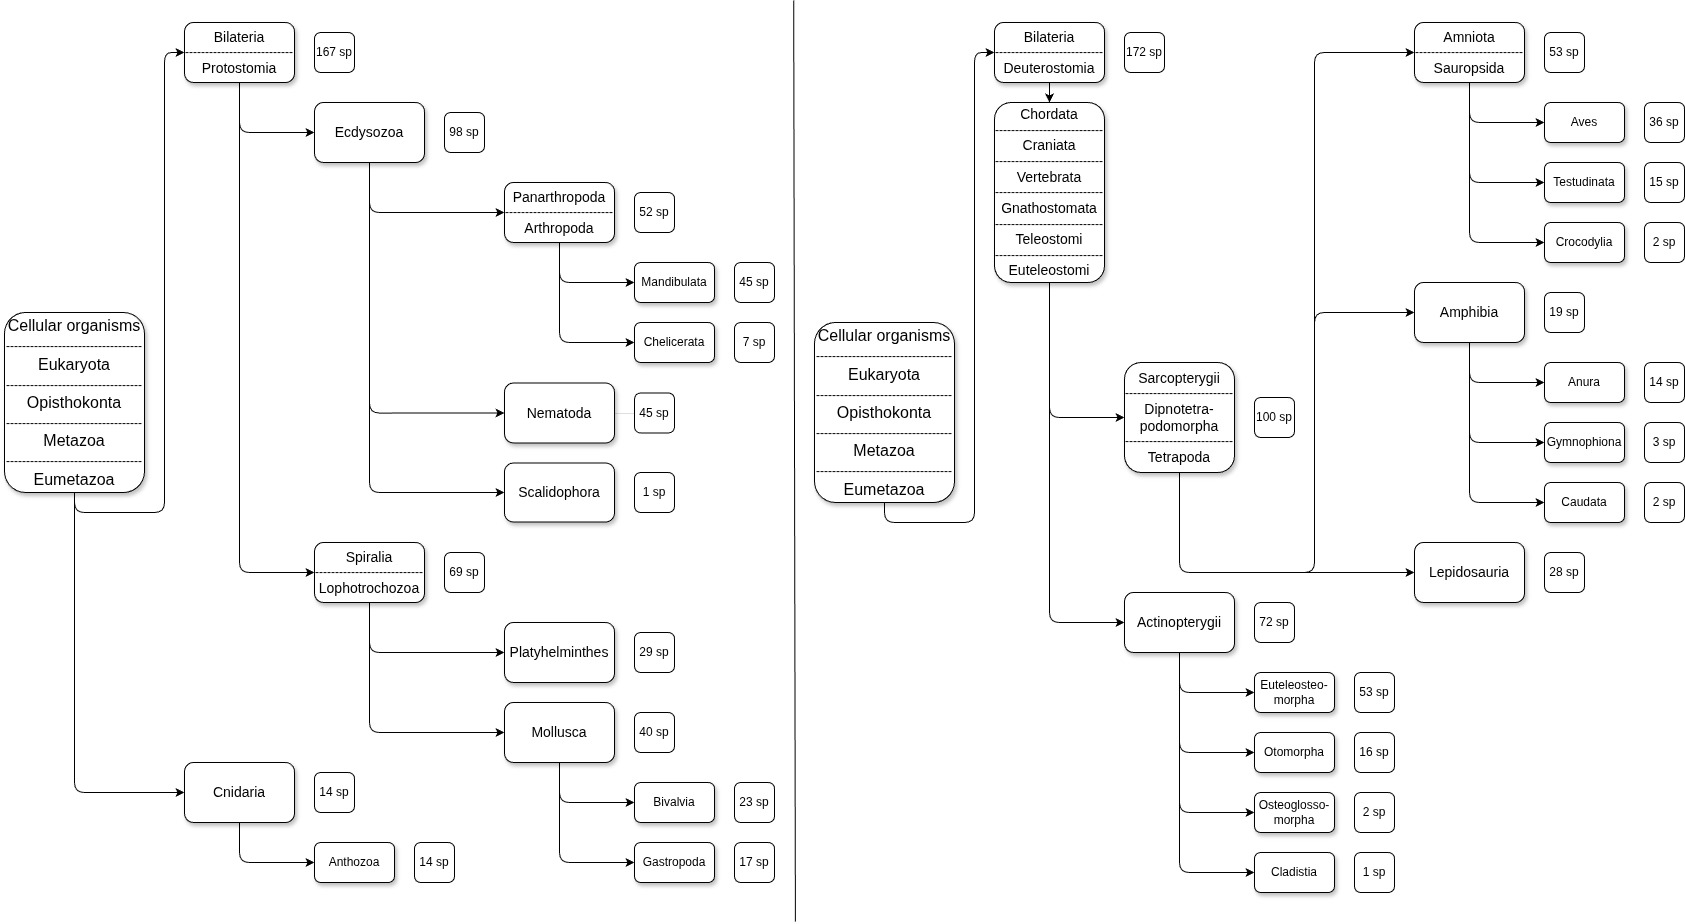
\includegraphics[width=1.0\textwidth]{images/Tree_summary}
    \caption{Количество видов, взятых в анализ, для разных таксономических групп.}
    \label{fig:tree_summary}
\end{figure}

Для всех видов, имеющих ``консервативную кассету``, были построены вторичные структуры для интрон-содержащего транскрипта с выделением цветом ``кассетного`` интрона.


\subsection{Подробный анализ Actinopterygii}

Для таксономической группы Actinopterygii проводился более углубленный анализ, так как на текущий момент данных по гену \textit{Nxf1} для них не было.
Были взяты все найденные нуклеотидные последовательности гена у представители данной филогенетической группы – 72 вида.


В таблице~\ref{tab:Actinopterygii} показана характеристика ``консервативной кассеты`` исследуемой группы.
Результаты по другим группам можно найти в приложении, таблицы~\ref{tab:Ecdysozoa}--\ref{tab:Lepidosauria}.

\begin{longtable}[c]{|c|c|c|c|c|}
\caption{Сводная таблица с характеристикой кассетного интрона для таксономической группы Actinopterygii.
Сортировка по возрастанию количества нуклеотидов до стоп-кодона в ``кассетном`` интроне.}
\label{tab:Actinopterygii}\\
\hline
\textbf{\begin{tabular}[c]{@{}c@{}}Название\\ организма\end{tabular}} &
  \textbf{\begin{tabular}[c]{@{}c@{}}Кол-во\\ нуклеотидов\\ до стоп-кодона\\ в интроне\end{tabular}} &
  \textbf{\begin{tabular}[c]{@{}c@{}}Длина\\ 1-го экзона\\ в кассете\end{tabular}} &
  \textbf{\begin{tabular}[c]{@{}c@{}}Длина\\ кассетного\\ интрона\end{tabular}} &
  \textbf{\begin{tabular}[c]{@{}c@{}}Длина\\ 2-го экзона\\ в кассете\end{tabular}} \\ \hline
\endfirsthead
%
\endhead
%
\hline
\endfoot
%
\endlastfoot
%
\textit{Chanos chanos}                 & 1   & 110 & 3568 & 37 \\
\textit{Danio rerio}                   & 1   & 110 & 3580 & 37 \\
\textit{Denticeps clupeoides}          & 7   & 110 & 2629 & 37 \\
\textit{Labrus bergylta}               & 10  & 110 & 2684 & 37 \\
\textit{Cottoperca gobio}              & 16  & 110 & 2388 & 37 \\
\textit{Xiphophorus couchianus}        & 22  & 110 & 2227 & 37 \\
\textit{Larimichthys crocea}           & 22  & 110 & 2340 & 37 \\
\textit{Lates calcarifer}              & 22  & 110 & 2434 & 37 \\
\textit{Notothenia coriiceps}          & 22  & 110 & 2886 & 37 \\
\textit{Betta splendens}               & 22  & 110 & 2274 & 37 \\
\textit{Poecilia reticulata}           & 22  & 110 & 2262 & 37 \\
\textit{Takifugu rubripes}             & 22  & 110 & 2114 & 37 \\
\textit{Salarias fasciatus}            & 22  & 110 & 3855 & 37 \\
\textit{Poecilia mexicana}             & 22  & 110 & 2247 & 37 \\
\textit{Stegastes partitus}            & 22  & 110 & 2900 & 37 \\
\textit{Clupea harengus}               & 22  & 110 & 3219 & 37 \\
\textit{Archocentrus centrarchus}      & 22  & 110 & 2644 & 37 \\
\textit{Esox lucius}                   & 22  & 110 & 2848 & 37 \\
\textit{Monopterus albus}              & 22  & 110 & 2353 & 37 \\
\textit{Echeneis naucrates}            & 22  & 110 & 2314 & 37 \\
\textit{Paralichthys olivaceus}        & 22  & 110 & 3148 & 37 \\
\textit{Maylandia zebra}               & 22  & 110 & 2565 & 37 \\
\textit{Parambassis ranga}             & 22  & 110 & 2484 & 37 \\
\textit{Sander lucioperca}             & 22  & 110 & 2494 & 37 \\
\textit{Xiphophorus maculatus}         & 22  & 110 & 2231 & 37 \\
\textit{Nothobranchius furzeri}        & 22  & 110 & 2290 & 37 \\
\textit{Anabas testudineus}            & 22  & 110 & 2352 & 37 \\
\textit{Acanthochromis polyacanthus}   & 22  & 110 & 2797 & 37 \\
\textit{Anarrhichthys ocellatus}       & 22  & 110 & 2355 & 37 \\
\textit{Boleophthalmus pectinirostris} & 22  & 110 & 1702 & 37 \\
\textit{Sparus aurata}                 & 22  & 110 & 2361 & 37 \\
\textit{Oryzias melastigma}            & 22  & 110 & 2212 & 37 \\
\textit{Seriola dumerili}              & 22  & 110 & 2494 & 37 \\
\textit{Poecilia formosa}              & 22  & 110 & 2259 & 37 \\
\textit{Oreochromis niloticus}         & 22  & 110 & 2580 & 37 \\
\textit{Kryptolebias marmoratus}       & 22  & 110 & 2556 & 37 \\
\textit{Xiphophorus hellerii}          & 22  & 110 & 2240 & 37 \\
\textit{Poecilia latipinna}            & 22  & 110 & 2261 & 37 \\
\textit{Pundamilia nyererei}           & 22  & 110 & 2527 & 37 \\
\textit{Hippocampus comes}             & 22  & 110 & 2622 & 37 \\
\textit{Oreochromis aureus}            & 22  & 110 & 2579 & 37 \\
\textit{Amphiprion ocellaris}          & 22  & 110 & 2752 & 37 \\
\textit{Seriola lalandi dorsalis}      & 22  & 110 & 2481 & 37 \\
\textit{Austrofundulus limnaeus}       & 22  & 110 & 2541 & 37 \\
\textit{Puntigrus tetrazona}           & 25  & 110 & 2440 & 37 \\
\textit{Fundulus heteroclitus}         & 25  & 110 & 2476 & 37 \\
\textit{Cyprinodon variegatus}         & 28  & 110 & 2533 & 37 \\
\textit{Haplochromis burtoni}          & 31  & 110 & 2535 & 37 \\
\textit{Astatotilapia calliptera}      & 31  & 110 & 2571 & 37 \\
\textit{Gouania willdenowi}            & 37  & 110 & 2616 & 37 \\
\textit{Oryzias latipes}               & 40  & 110 & 2331 & 37 \\
\textit{Sphaeramia orbicularis}        & 43  & 110 & 2376 & 37 \\
\textit{Pygocentrus nattereri}         & 46  & 110 & 2649 & 37 \\
\textit{Astyanax mexicanus}            & 46  & 110 & 2791 & 37 \\
\textit{Colossoma macropomum}          & 46  & 110 & 2644 & 37 \\
\textit{Ictalurus punctatus}           & 46  & 110 & 3166 & 37 \\
\textit{Tachysurus fulvidraco}         & 46  & 110 & 3493 & 37 \\
\textit{Pangasianodon hypophthalmus}   & 46  & 110 & 3348 & 37 \\
\textit{Erpetoichthys calabaricus}     & 55  & 110 & 3662 & 37 \\
\textit{Perca flavescens}              & 58  & 110 & 2378 & 37 \\
\textit{Mastacembelus armatus}         & 64  & 110 & 2371 & 37 \\
\textit{Salmo salar}                   & 67  & 110 & 3553 & 37 \\
\textit{Gadus morhua}                  & 67  & 110 & 3151 & 37 \\
\textit{Etheostoma spectabile}         & 97  & 110 & 2457 & 37 \\
\textit{Scleropages formosus}          & 112 & 110 & 3412 & 37 \\
\textit{Myripristis murdjan}           & 112 & 110 & 2492 & 37 \\
\textit{Paramormyrops kingsleyae}      & 121 & 110 & 2929 & 37 \\
\textit{Carassius auratus}             & 148 & 110 & 3854 & 37 \\
\textit{Sinocyclocheilus grahami}      & 148 & 110 & 3330 & 37 \\
\textit{Sinocyclocheilus rhinocerous}  & 154 & 110 & 3449 & 37 \\
\textit{Sinocyclocheilus anshuiensis}  & 154 & 110 & 4202 & 37 \\
\textit{Electrophorus electricus}      & 283 & 110 & 2874 & 37 \\ \hline
\end{longtable}


На рисунках~\ref{fig:Actinopterygii_intron_stop} и~\ref{fig:Actinopterygii_intron} показано распределение длин части ``кассетного`` интрона до стоп-кодона и длин ``кассетного`` интрона, соответственно.

\begin{figure}[h] % here, top, bottom, page
    \centering
    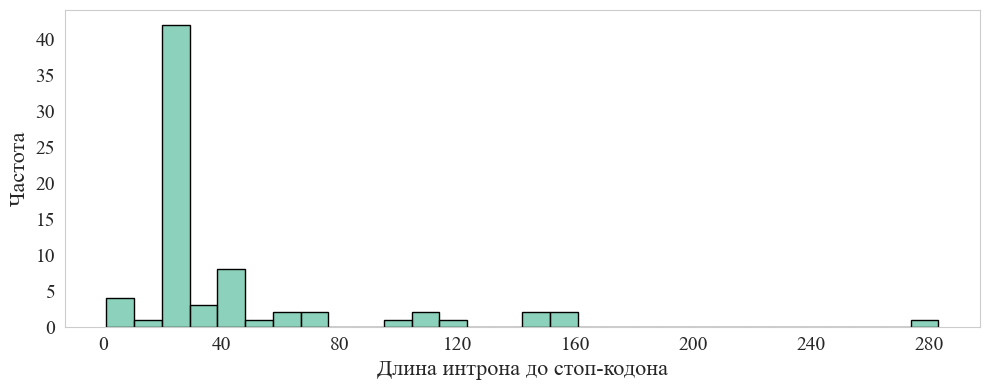
\includegraphics[width=1.0\textwidth]{images/Actinopterygii_intron_stop}
    \caption{Распределение длин части ``кассетного`` интрона до стоп-кодона у Actinopterygii}
    \label{fig:Actinopterygii_intron_stop}
\end{figure}

\begin{figure}[h] % here, top, bottom, page
    \centering
    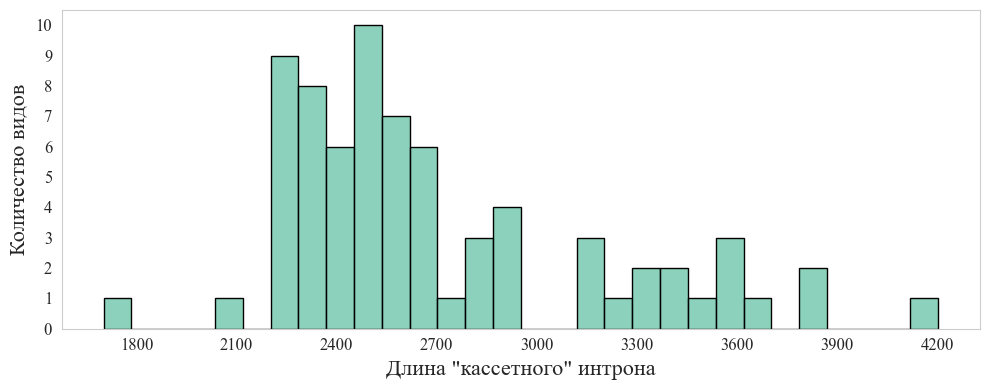
\includegraphics[width=1.0\textwidth]{images/Actinopterygii_intron}
    \caption{Распределение длин ``кассетного`` интрона у Actinopterygii}
    \label{fig:Actinopterygii_intron}
\end{figure}


На рисунке~\ref{fig:Actinopterygii_maxentscan} представлены результаты оценки ``силы сайтов сплайсинга`` - ``ящики с усами``, отображающие распределение MaxEntScan score для таксонов более низкого ранга внутри группы Actinopterygii.
Разбиение на подгруппы основано на их удаленности друг от друга.
Порядок групп на графике не несет смысловой нагрузки.

\begin{figure}[h] % here, top, bottom, page
    \centering
    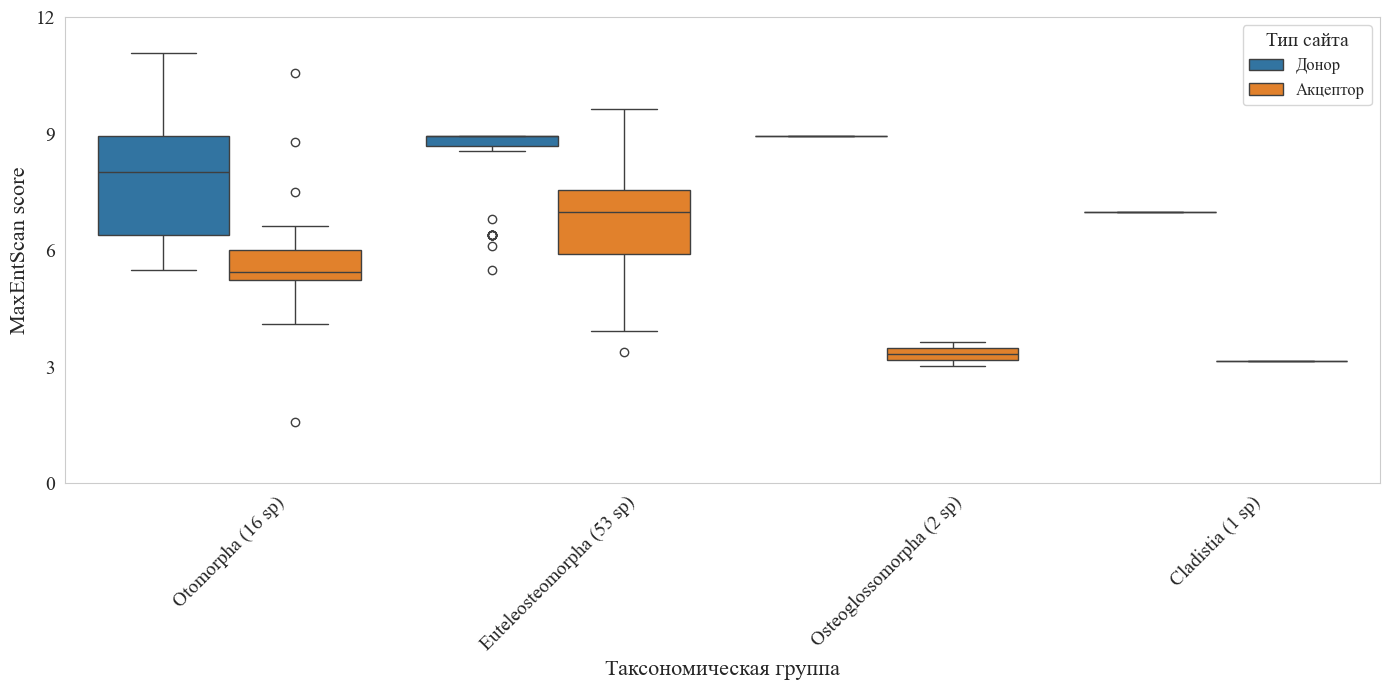
\includegraphics[width=1.0\textwidth]{images/Actinopterygii_maxentscan}
    \caption{Результаты проведения MaxEntScan для Actinopterygii.}
    \label{fig:Actinopterygii_maxentscan}
\end{figure}


Рисунок~\ref{fig:Actinopterygii_meme} демонстрирует результаты, полученные с помощью MEME Suite.

Найденные мотивы присутствуют не у всех видов, взятых в анализ изначально, их количество отображено в столбце Sites.
Нас заинтересовал 2-й найденный мотив, так как его начало схоже с предложенной авторами~\cite{cte_consensus} консенсусной последовательностью для CTE из рисунка~\ref{fig:CTE_consensus}.
К сожалению, использование Tomtom для сравнения найденных консервативных мотивов из ``кассетного`` интрона с базой данных не дало статистически значимых результатов.

\begin{figure}[h] % here, top, bottom, page
    \centering
    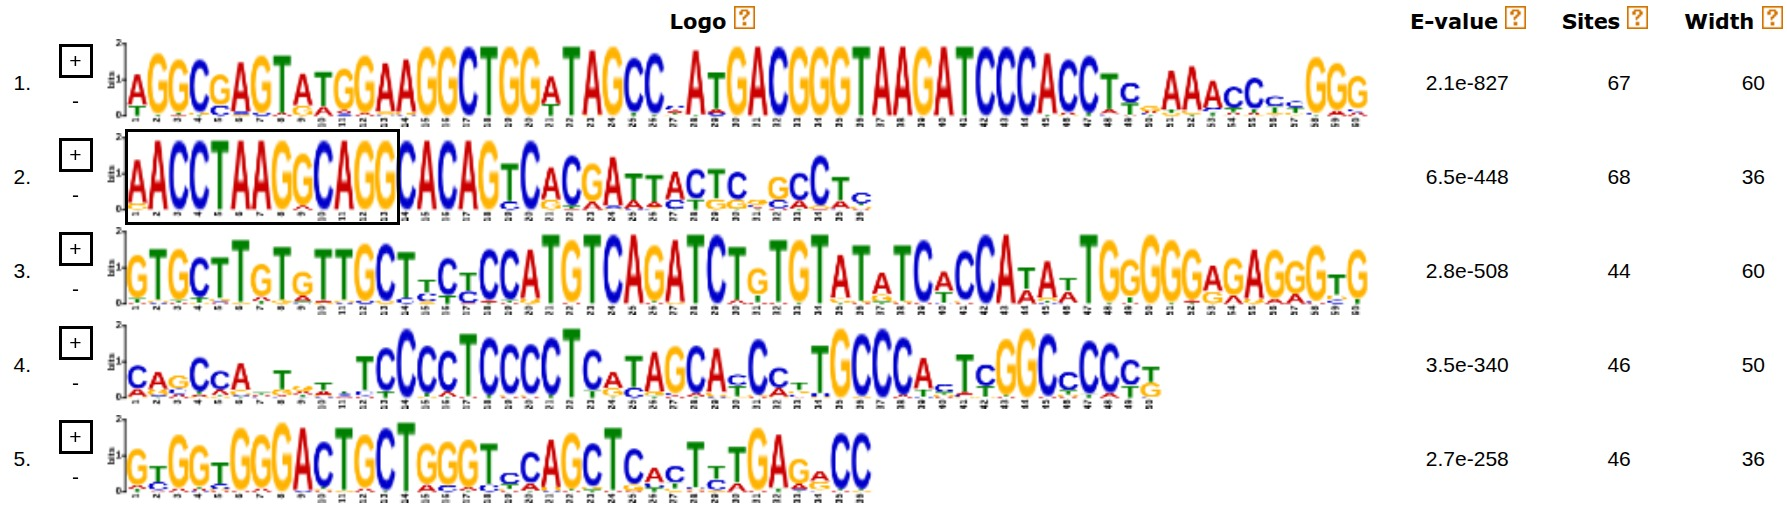
\includegraphics[width=1.0\textwidth]{images/Actinopterygii_meme_motif}
    \caption{Результат поиска мотивов внутри ``кассетного`` интрона с помощью MEME Suite для Actinopterygii. Черным прямоугольником выделен участок, похожий на консенсусную последовательность CTE (рис.~\ref{fig:CTE_consensus})~\cite{cte_consensus}}
    \label{fig:Actinopterygii_meme}
\end{figure}.

\begin{figure}[H] % here, top, bottom, page
    \centering
    
\includegraphics[width=0.7\textwidth]{images/CTE_consensus}
    \caption{Консенсусный конститутивный транспортный элемент (CTE)~\cite{cte_consensus}.}
    \label{fig:CTE_consensus}
\end{figure}

\vspace{1cm}

Репрезентация вторичной структуры интрон-содержащего транскрипта с выделенным кассетным интроном и найденным мотивом показана на рисунке~\ref{fig:Chanos_chanos_2nd_structure}.
У всех видов были сходные структуры и в качестве иллюстрации представлен один из проанализированных видов.

Учитывая тот факт, что мотив с интересующим нас участком, был найден у 68 видов, именно для них был проведен последующий анализ.

Рисунок~\ref{fig:Actinopterygii_alignment_ruler} отображает результаты множественного выравнивания, а на рисунке~\ref{fig:Actinopterygii_tree} представлено филогенетическое дерево, построенное по результатам этого выравнивания.

\begin{sidewaysfigure}
    \centering
    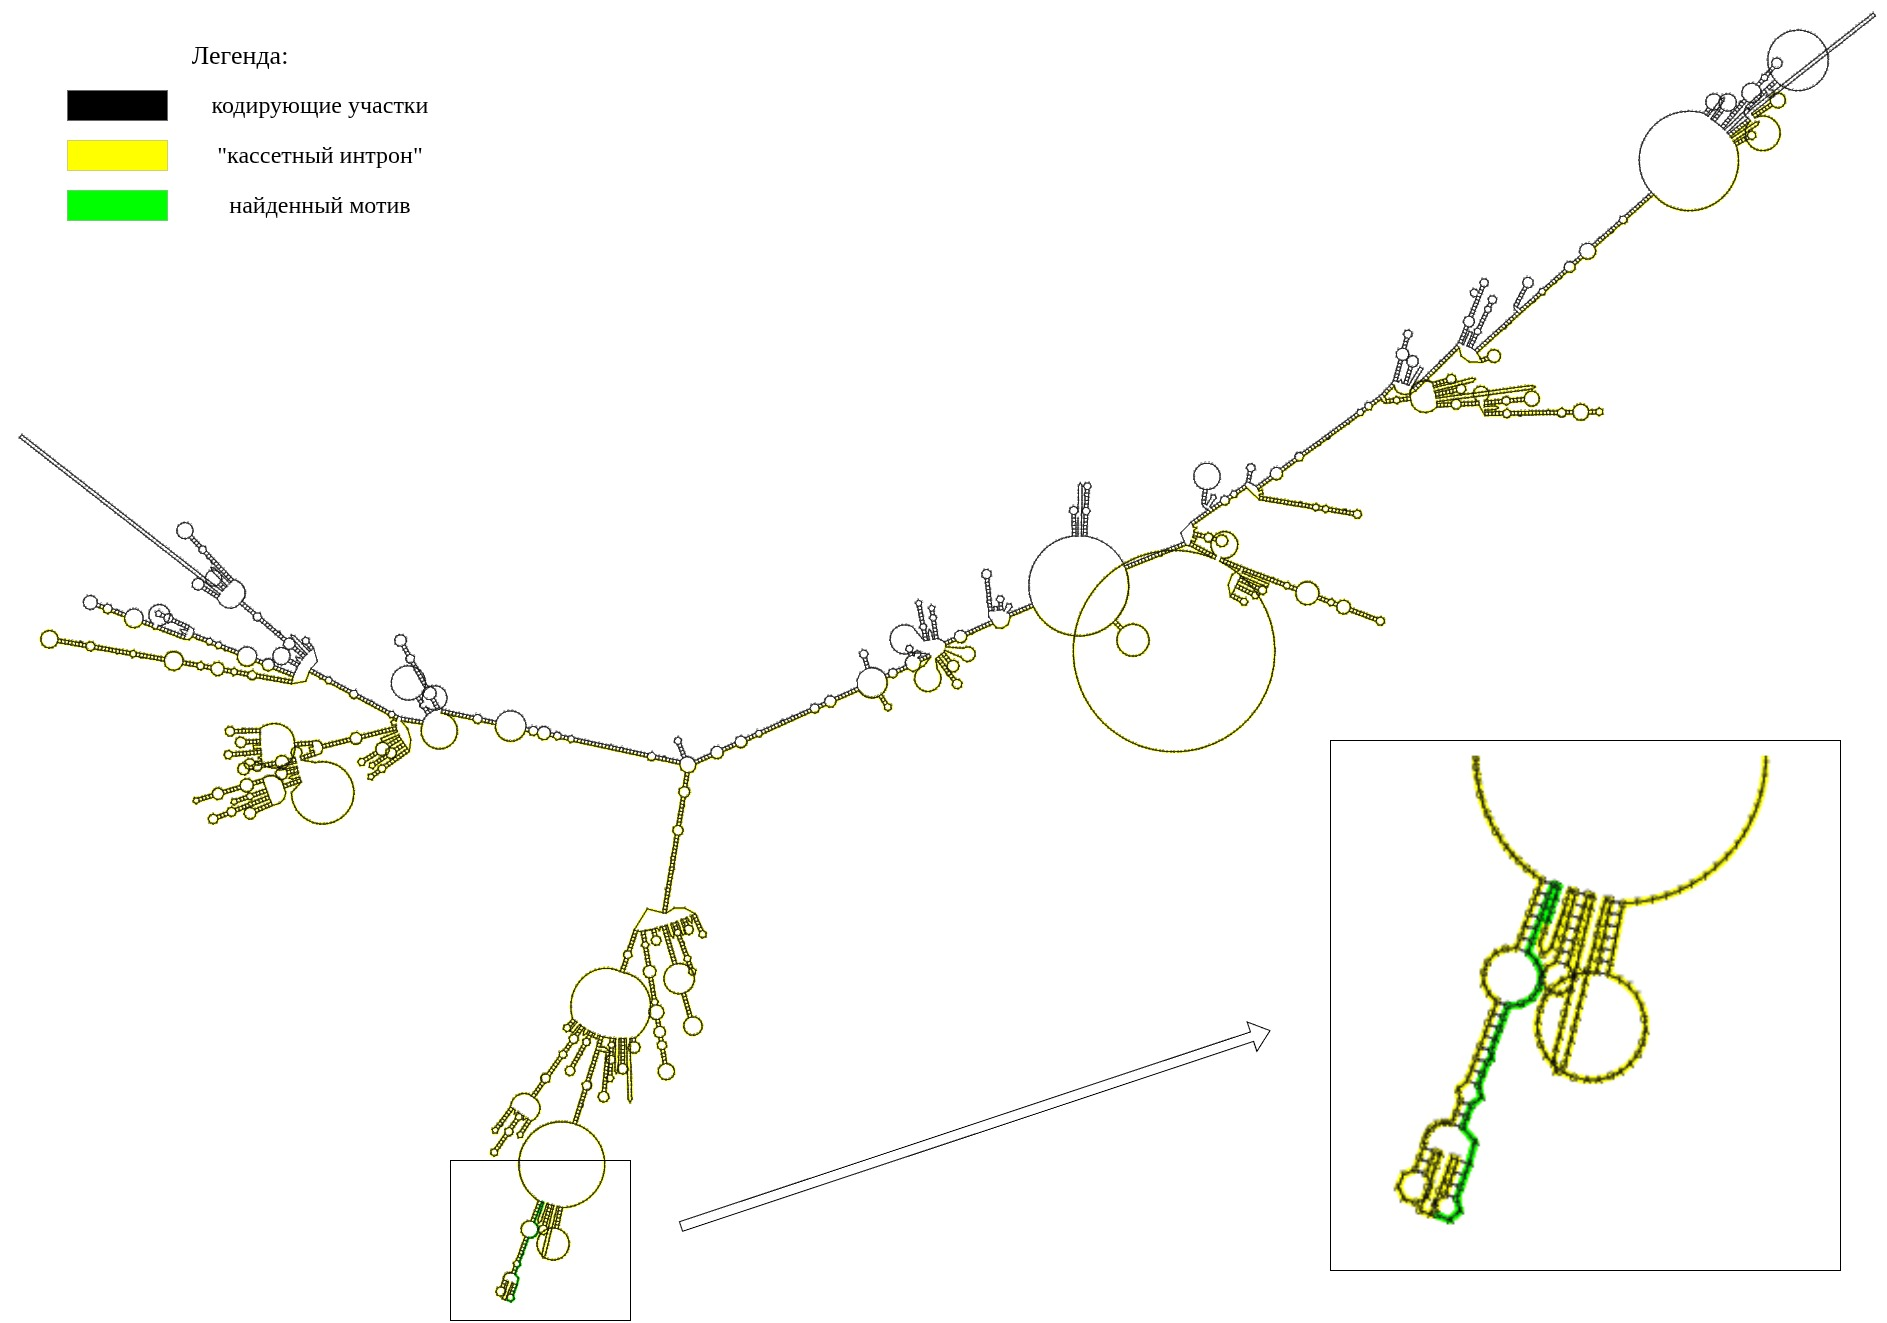
\includegraphics[width=0.9\textheight]{images/Chanos_chanos_2nd_structure}
    \caption{Вторичная структура РНК-транскрипта для \textit{Chanos chanos} из Otomorpha, содержащая ``кассетный`` интрон.}
    \label{fig:Chanos_chanos_2nd_structure}
\end{sidewaysfigure}

\begin{figure}[ht] % here, top, bottom, page
    \centering
    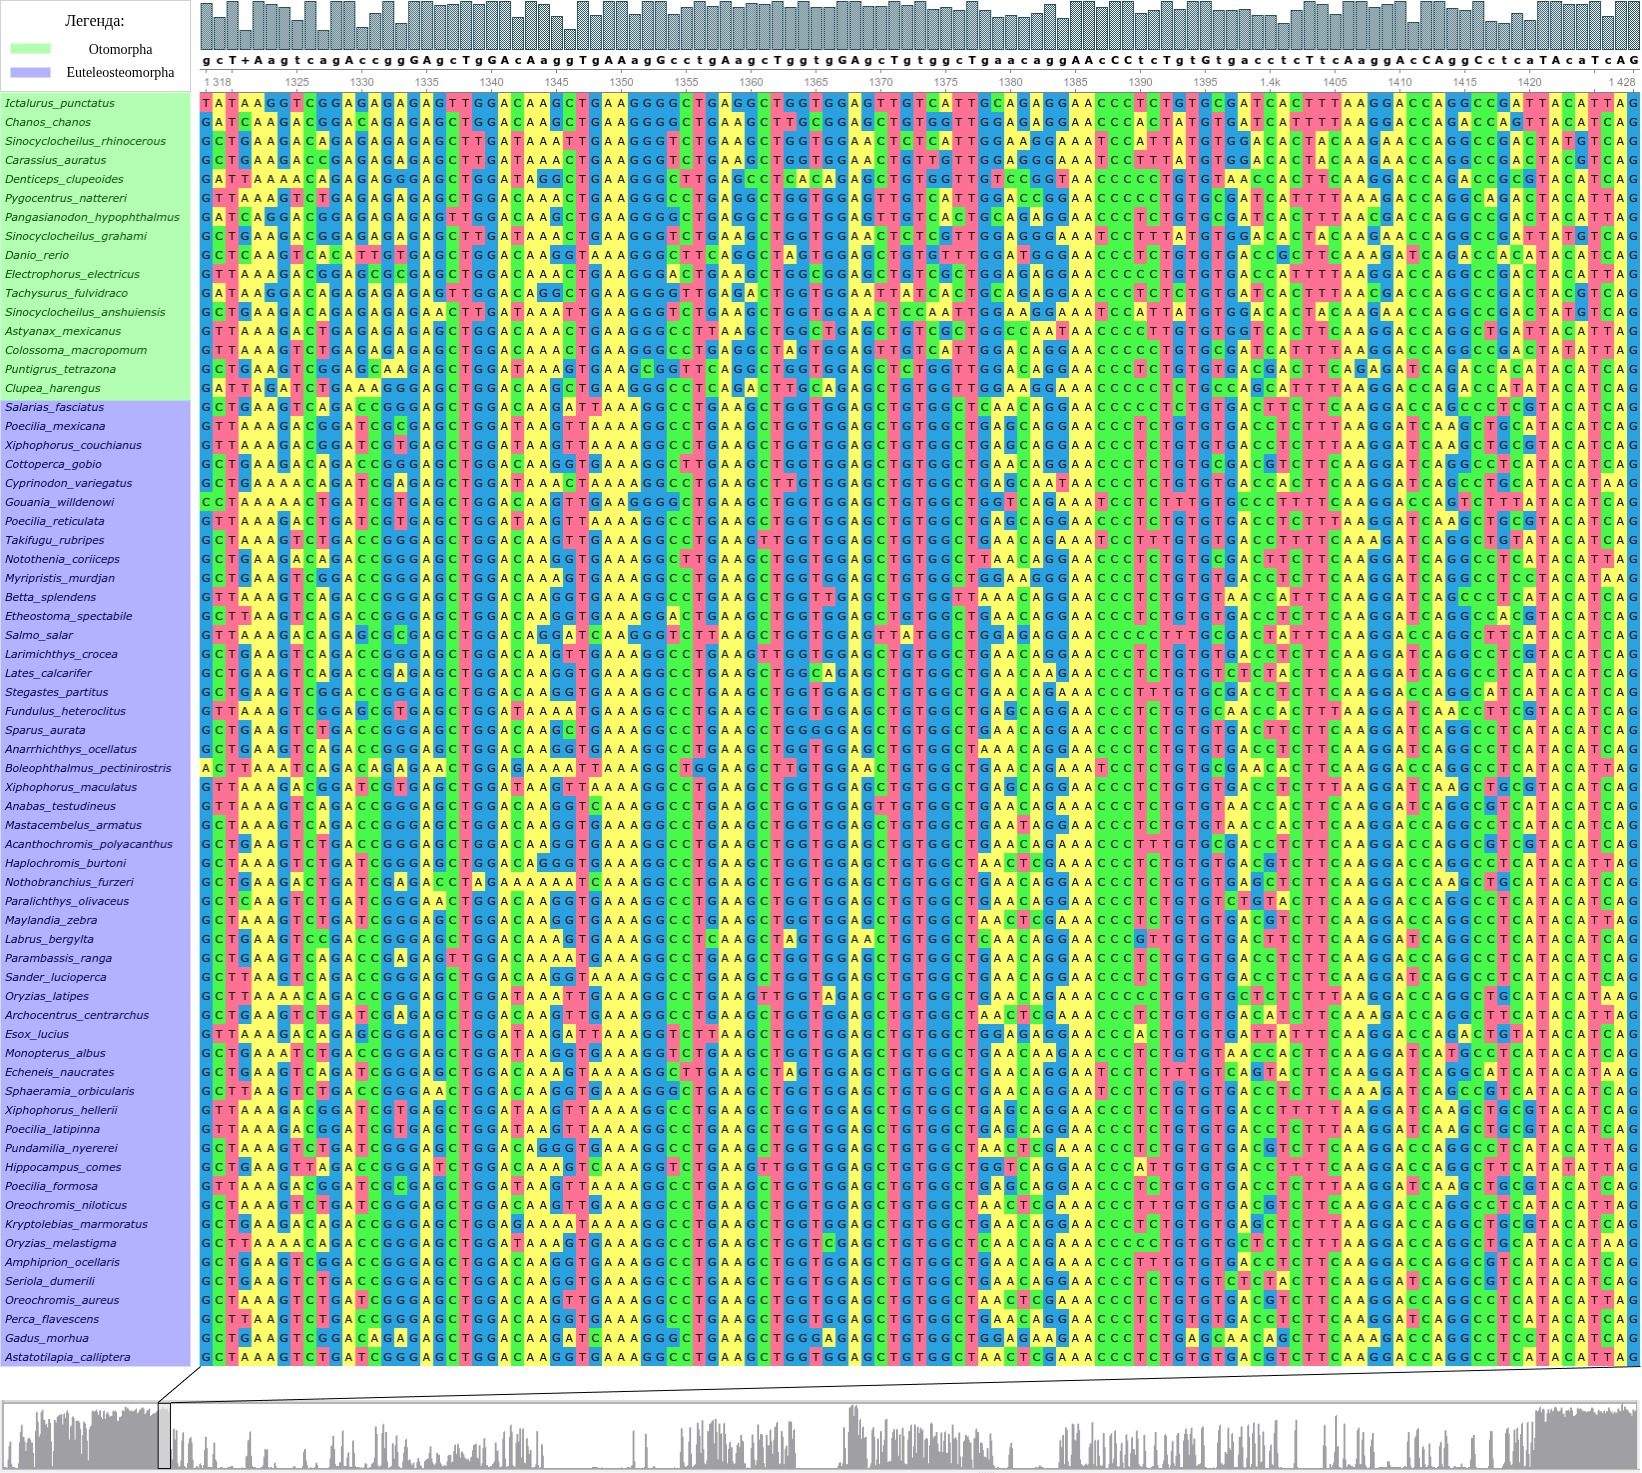
\includegraphics[width=0.9\textwidth]{images/Actinopterygii_alignment_ruler}
    \caption{Результаты множественного выравнивания для Actinopterygii.}
    \label{fig:Actinopterygii_alignment_ruler}
\end{figure}

\begin{figure}[hb] % here, top, bottom, page
    \centering
    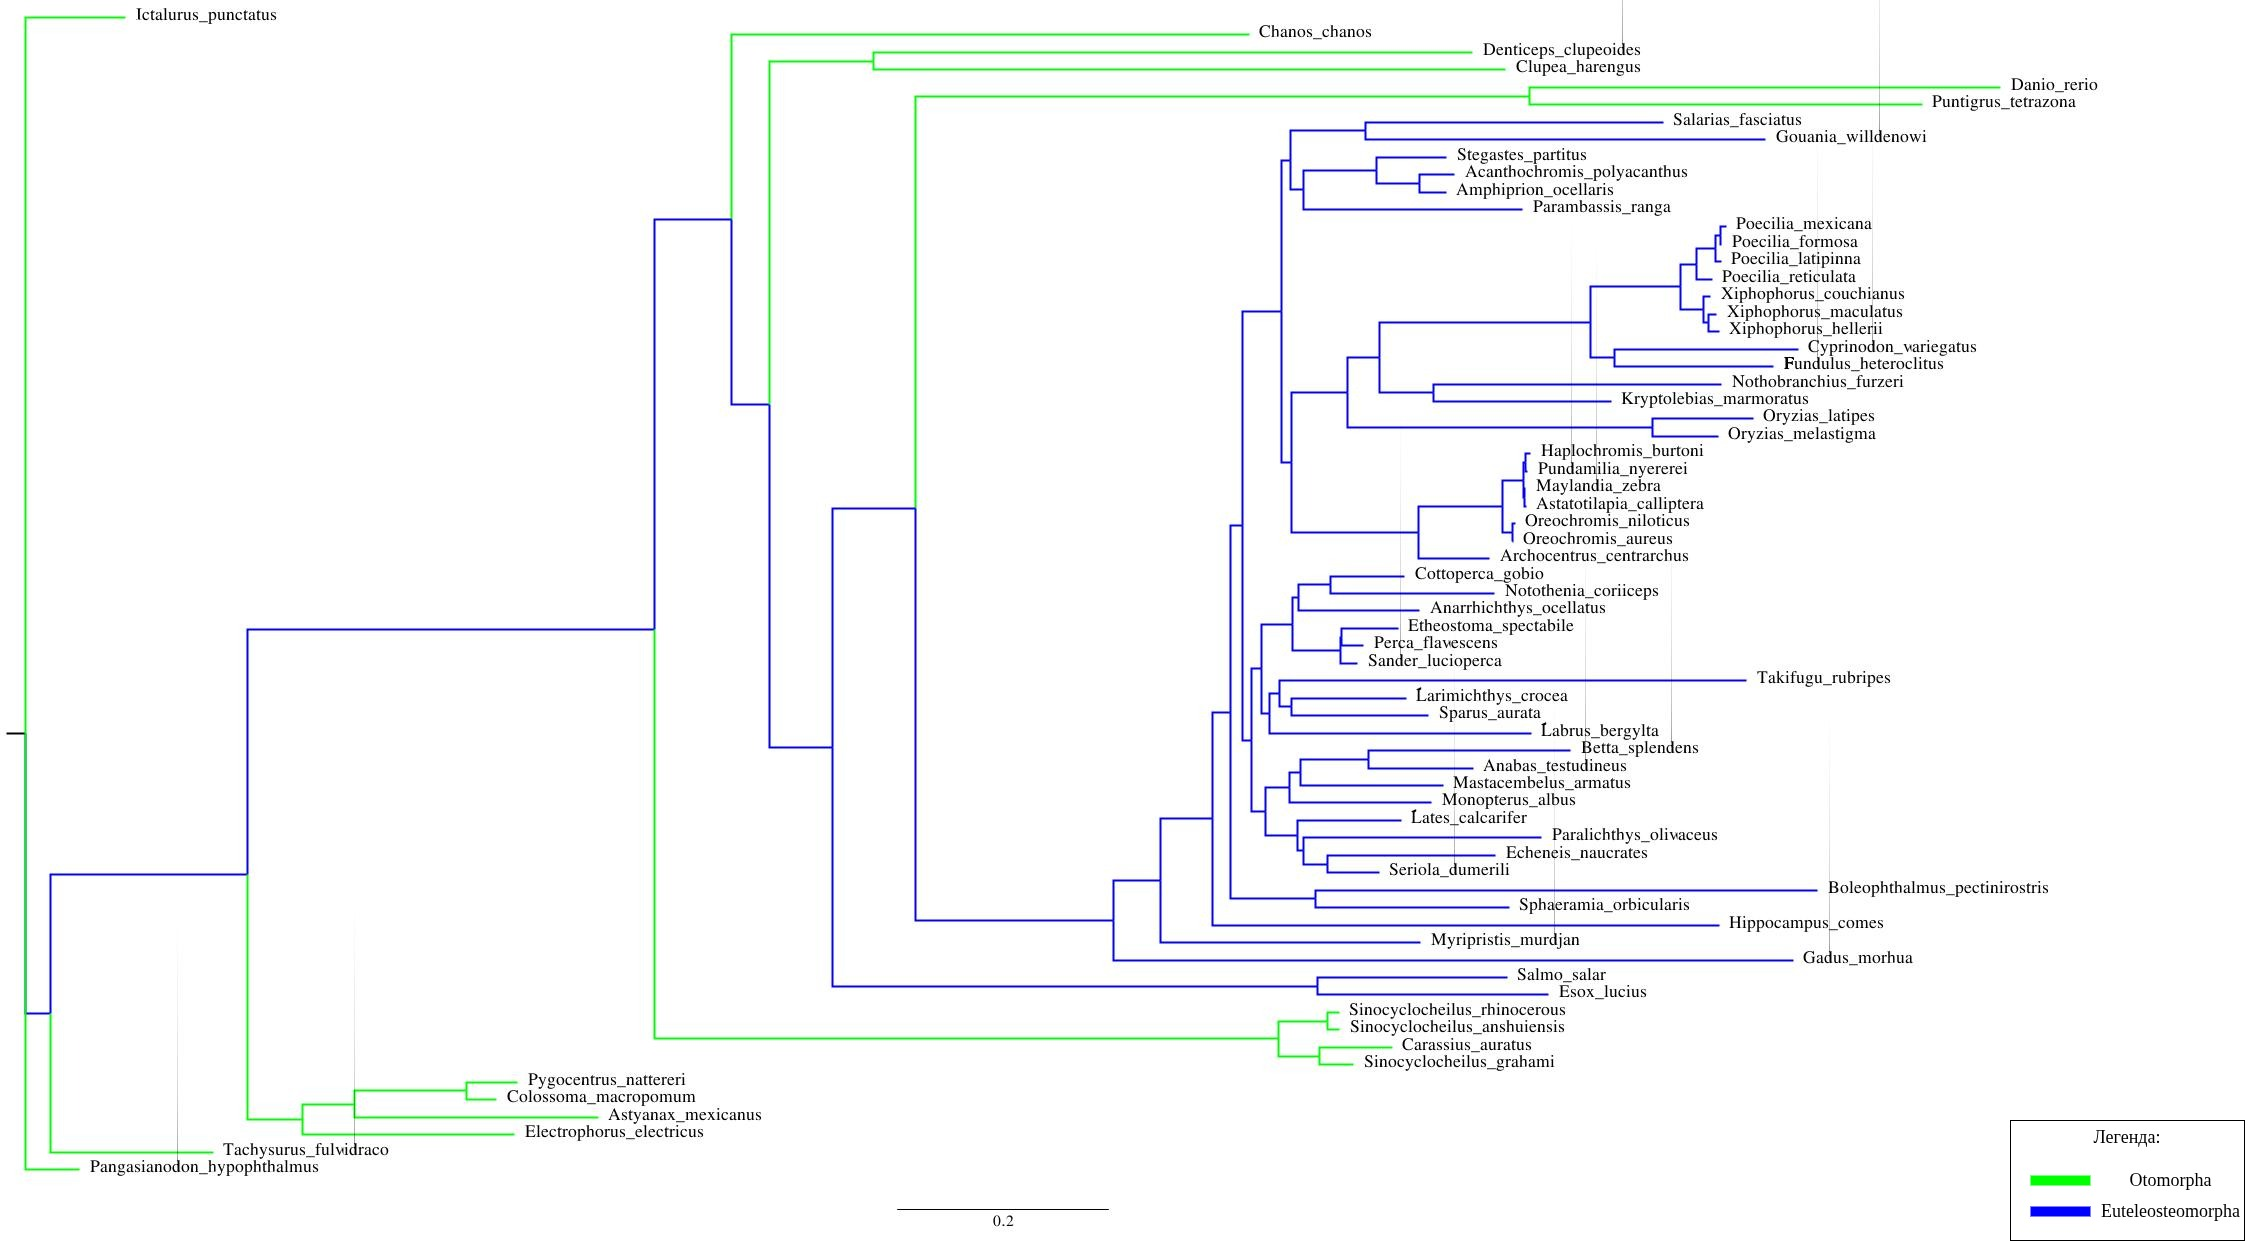
\includegraphics[width=1.0\textwidth]{images/Actinopterygii_tree}
    \caption{Филогенетическое дерево для Actinopterygii.}
    \label{fig:Actinopterygii_tree}
\end{figure}

% Обсуждение
\clearpage
\section{Обсуждение}

\subsection{Анализ всех найденных видов}

У всех проанализированных видов размер второго экзона из ``консервативной кассеты`` равен 37 нуклеотидам, в то время как размер первого экзона варьирует в различных группах (см. таблицу~\ref{tab:Comparison_groups}).
На рисунке~\ref{fig:Protostomia_exon} показано распределение длины первого экзона из ``кассеты`` для Protostomia.

\begin{figure}[h] % here, top, bottom, page
    \centering
    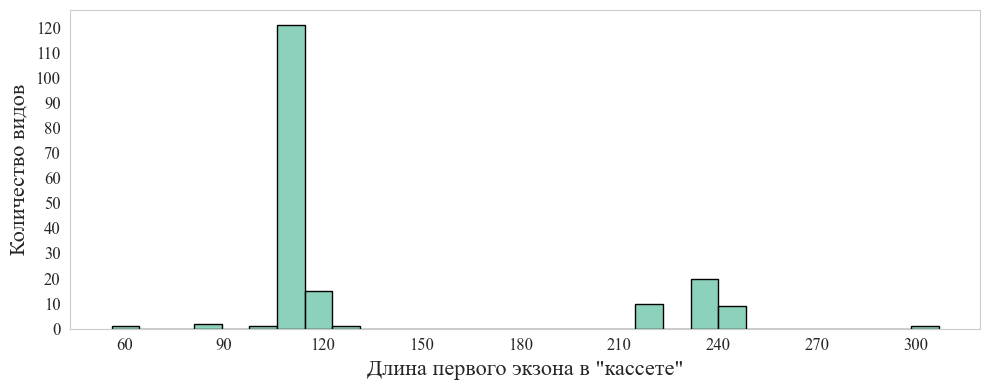
\includegraphics[width=0.9\textwidth]{images/Protostomia_exon}
    \caption{Распределение длины первого экзона из ``консервативной кассеты`` для Protostomia.}
    \label{fig:Protostomia_exon}
\end{figure}

Для Ecdysozoa и Cnidaria первый экзон как правило размером 110 нуклеотидов, но встречаются и исключения.
У Spiralia размер этого экзона гораздо больше и чаще всего составляет 239 нуклеотидов.
По данному отличию и встречающимся уникальным вариантам размера экзона требуется углубленное исследование.

У Deuterostomia размер первого экзона в абсолютном большинстве случаев (171 из 172 исследованных видов) составляет 110 нуклеотидов, что также характерно и для млекопитающих.

Длина участка внутри интрона до стоп-кодона, как и длина самого интрона, варьирует в более широких пределах в разных группах.
Тем не менее внутри отдельных групп, например Lepidosauria (таблица~\ref{tab:Lepidosauria} в приложении), наблюдается высокая степень консервативности обоих параметров.

Также встречаются виды, у которых происходит частичная или даже полная трансляция ``кассетного`` интрона, потому что в нем не встречается преждевременный стоп-кодон.
Например, таким видом является давно изученная в данном контексте \textit{Caenorhabditis elegans}, у которой преждевременный стоп-кодон встречается в одном из экзонов после ``кассетного`` интрона.
В данном исследовании были найдены еще 2 вида, у которых интрон полностью считывается: Aves – \textit{Vidua chalybeata}, Paraneoptera – \textit{Rhopalosiphum maidis}.
Упомянутые виды также требуют тщательного изучения.


\subsection{Подробный анализ Actinopterygii}

Данная группа организмов была исследована более подробно по перечисленным ранее причинам.
Внутри группы размеры первого и второго экзона из ``консервативной кассеты`` для всех исследованных видов составляют 110 и 37 нуклеотидов, соответственно.
Длина участка внутри интрона до стоп-кодона у большинства видов составляет 22 нуклеотида (39 из 72 исследованных в работе).
Размер ``кассетного`` интрона варьирует от 1702 до 4202 нуклеотидов (медиана – 2549).

Анализ ``сайтов силы сплайсинга`` (рис.~\ref{fig:Actinopterygii_maxentscan}) говорит о том, что у всех исследованных видов в работе данный интрон успешно вырезается сплайсосомой.
Учитывая большую выборку видов, взятую для анализа, было принято решение ориентироваться на эмпирическую интерпретацию результатов, которая выглядит следующим образом:

\begin{spacing}{0.5}
\begin{itemize}
    \item 0–3: слабый сайт сплайсинга
    \item 3–6: умеренный сайт сплайсинга
    \item >6: сильный сайт сплайсинга
\end{itemize}
\end{spacing}

Так как у большинства видов значение MaxEntScan score больше или около 6, был сделан вывод, высказанный выше.
Соответственно, удержание интрона является не ошибкой сплайсинга, а закономерным событием варианта альтернативного сплайсинга.
В связи с этим и было принято решение о поиске консервативных мотивов внутри ``кассетного`` интрона.

Несмотря на то, что на рисунке~\ref{fig:Actinopterygii_meme} представлено 5 найденных мотивов, их количество может быть больше, потому что данное значение мотивов было ограничением запуска MEME Suite.
Учитывая высокую степень сходства начала 2-го найденного мотива с консенсусной последовательностью CTE из рисунка~\ref{fig:CTE_consensus}, можно предположить сохранение интрона благодаря этой и возможно другим структурам внутри интрон-содержащего транскрипта (рис.~\ref{fig:Chanos_chanos_2nd_structure}).
Было бы интересно узнать, как именно CTE-подобная последовательность оказалось в данном интроне.

Проведенное множественное выравнивание на рисунке~\ref{fig:Actinopterygii_alignment_ruler} говорит о высокой степени консервативности как кодирующих участков – левый и правый крайние части диаграммы под выравниванием, так и некоторых участков внутри интрона – центр диаграммы под выравниванием.

Филогенетическое древо (рис.~\ref{fig:Actinopterygii_tree}), построенное по результатам выравнивания, несмотря на наличие ``кассетного`` интрона в последовательности, использованной для его построения, успешно разделяет виды на таксоны более высокого ранга – Otomorpha и Euteleosteomorpha.

Остальные группы, не включенные в подробный анализ, требуют его проведения.

% Выводы
% \clearpage
\section{Выводы}

\begin{enumerate}[left=\parindent]
    \item Внутри одной таксономической группы существуют преобладающие значения для характеристик ``консервативной кассеты``:
    \begin{itemize}
        \item длина первого и второго экзона;
        \item длина ``кассетного`` интрона;
        \item длина участка внутри ``кассетного`` интрона до стоп-кодона.
    \end{itemize}
    \item Внутри ``кассетного`` интрона существуют участки, которые образуют особые структуры при формировании вторичной структуры интрон-содержащего транскрипта, и за счет их наличия возможно сохранение такого транскрипта и последующая трансляция с синтезом укороченной формы белка.
\end{enumerate}


% Список литературы
\newpage
\section{Список литературы}
\printbibliography[heading=none]


% Благодарности
% \clearpage
\section{Благодарности}

Я хотел бы поблагодарить моего научного руководителя, Голубкову Елену Валерьевну, и моего куратора, Бондарука Дмитрия Денисовича, за постоянную поддержку и помощь в обсуждении результатов работы.

Отдельно я хотел бы поблагодарить Абрамсон Наталью Иосифовну за повторное рецензирование работы моего авторства.

Также хочу выразить благодарность преподавателям программы ``Биоинформатика`` и кафедры генетики и биотехнологии СПбГУ, и коллективу преподавателей и ассистентов Института Биоинформатики за полученные знания в процессе обучения, с помощью которых стало возможным осуществление данной работы.

% Приложение (может быть пустым)
% \clearpage
\section{Приложение}



\end{document}
